\chapter{TOOLS AND TECHNOLOGIES}

\hs This chapter presents the main tools, libraries, and technologies used in the development and implementation of the proposed \KFCProcedure{} and \GradientCOBRA{} frameworks. The system was implemented in Python and relied on several scientific computing, machine learning, visualization, and development tools to support data processing, model training, aggregation, evaluation, experimentation, and reproducibility.

\section{Programming Language}

\begin{figure}[H]
    \centering
    
\includegraphics[width=0.25\textwidth]{figures/tools/python.png}
    \caption{Python Programming Language}
    \label{fig:python}
\end{figure}

\hs As shown in Figure~\ref{fig:python}, the entire system was implemented using Python, which is widely used in machine learning research due to its simplicity, readability, and extensive ecosystem of scientific libraries. Python provides strong support for numerical computation, data manipulation, and machine learning model development, making it suitable for implementing both the \KFCProcedure{} and \GradientCOBRA{} frameworks.

\section{Machine Learning and Scientific Computing Libraries}

\hs The proposed system was implemented using a set of machine learning and scientific computing libraries in Python. These libraries provided the fundamental building blocks for data processing, model development, optimization, and evaluation in both the \KFCProcedure{} and \GradientCOBRA{} frameworks. Each library played a specific role in ensuring computational efficiency, modularity, and scalability of the system.

\subsection{NumPy}

\begin{figure}[H]
    \centering
    \includegraphics[width=0.25\textwidth]{figures/tools/NumPy.png}
    \caption{NumPy in Scientific Computing}
    \label{fig:numpy}
\end{figure}

\hs As shown in Figure~\ref{fig:numpy}, NumPy was used as the core numerical computing library in the system. It provides efficient support for multidimensional arrays, linear algebra operations, and vectorized computations. In the proposed frameworks, NumPy was primarily used for handling dataset representations, prediction matrices, distance computations, and mathematical transformations required in both clustering and aggregation processes.

\subsection{Scikit-learn}

\begin{figure}[H]
    \centering
    
\includegraphics[width=0.25\textwidth]{figures/tools/sklearn.png}
    \caption{Scikit-learn Machine Learning Framework}
    \label{fig:sklearn}
\end{figure}

\hs As shown in Figure~\ref{fig:sklearn}, Scikit-learn was used as the primary machine learning library for implementing base estimators, preprocessing utilities, and evaluation metrics. It provides a wide range of regression and classification models that can be integrated into both the \KFCProcedure{} and \GradientCOBRA{} frameworks. Additionally, it supports data splitting, scaling, and performance evaluation, which are essential for experimental validation.

\subsection{SciPy}

\begin{figure}[H]
    \centering
    \includegraphics[width=0.25\textwidth]{figures/tools/SciPy.png}
    \caption{SciPy Scientific Computing Library}
    \label{fig:scipy}
\end{figure}

\hs As shown in Figure~\ref{fig:scipy}, SciPy was used for advanced mathematical operations and optimization-related computations. It supports statistical functions, numerical integration, and optimization routines that are useful in the \GradientCOBRA{} framework, particularly in kernel transformations and loss-related computations.

\subsection{Joblib}

\begin{figure}[H]
    \centering
    
\includegraphics[width=0.25\textwidth]{figures/tools/joblib.png}
    \caption{Joblib Parallel Processing Utility}
    \label{fig:joblib}
\end{figure}

\hs As shown in Figure~\ref{fig:joblib}, Joblib was used for model persistence and efficient computation through parallel processing. In the proposed system, it supported saving trained models and improving execution efficiency when handling multiple estimators or clusterwise models in \KFCProcedure{}.

\subsection{Summary of Machine Learning and Scientific Computing Libraries}

\hs Overall, these libraries formed the computational backbone of the proposed system. NumPy provided numerical efficiency, Scikit-learn enabled machine learning modeling, SciPy supported mathematical optimization, and Joblib enhanced performance and scalability. The integration of these libraries ensured that both \KFCProcedure{} and \GradientCOBRA{} could be implemented in a modular, efficient, and reproducible manner.

\section{Development Environment}

\hs The development environment defined the software tools and platforms used to implement, test, and execute the proposed \KFCProcedure{} and \GradientCOBRA{} frameworks. A well-structured development environment was essential for ensuring reproducibility, efficient debugging, and smooth experimentation during model development. In this study, the system was developed using Python-based tools combined with modern code editors and notebook environments.

The primary development environment included an integrated development environment for code writing and debugging, as well as an interactive notebook interface for experimentation and visualization. These tools supported iterative development, allowing rapid testing of clustering methods, predictive models, and optimization strategies. In addition, version control tools were used to manage code changes and maintain project consistency throughout development.

\subsection{Visual Studio Code}

\begin{figure}[H]
    \centering
    
\includegraphics[width=0.25\textwidth]{figures/tools/vscode.png}
    \caption{Visual Studio Code Integrated Development Environment}
    \label{fig:vscode}
\end{figure}

As shown in Figure~\ref{fig:vscode}, Visual Studio Code was used as the main integrated development environment for implementing the proposed system. This IDE provides features such as syntax highlighting, debugging tools, code navigation, and extension support, which improve development efficiency. It was particularly useful for managing the modular structure of both the \KFCProcedure{} and \GradientCOBRA{} packages.

\subsection{Jupyter Notebook}

\begin{figure}[H]
    \centering
    \includegraphics[width=0.25\textwidth]{figures/tools/jupyter.png}
    \caption{Jupyter Notebook Environment}
    \label{fig:jupyter}
\end{figure}

As shown in Figure~\ref{fig:jupyter}, Jupyter Notebook was used for experimental development, testing, and visualization of intermediate results. It allowed step-by-step execution of code, making it suitable for validating clustering outputs, model predictions, and optimization behavior. This environment was especially useful for comparing different configurations of \GradientCOBRA{} and \KFCProcedure{} in an interactive manner.

\subsection{Google Colab}

\begin{figure}[H]
    \centering
    
\includegraphics[width=0.25\textwidth]{figures/tools/colab.png}
    \caption{Google Colab Environment}
    \label{fig:colab}
\end{figure}

As shown in Figure~\ref{fig:colab}, Google Colab was used as a cloud-based notebook environment for running experiments and validating the behavior of the proposed frameworks. It provided an accessible Python execution environment with pre-installed scientific computing libraries and support for interactive experimentation. In this study, Google Colab was useful for executing experimental workflows, testing model configurations, and generating intermediate outputs without requiring a complex local setup. It complemented Jupyter Notebook by providing a flexible cloud platform for experimentation and reproducibility.

\subsection{Version Control System}

\begin{figure}[H]
    \centering
    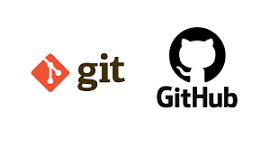
\includegraphics[width=0.5\textwidth]{figures/tools/git.png}
    \caption{Git and GitHub Workflow}
    \label{fig:git}
\end{figure}

As shown in Figure~\ref{fig:git}, Git and GitHub were used for version control and source code management throughout the development of the system. Git was used locally to track changes in the codebase, manage different versions of the project, and enable rollback to previous states when necessary. GitHub was used as a remote repository hosting platform to store the project, maintain backups, and facilitate collaboration and version synchronization. This combination ensured that the development of both the \KFCProcedure{} and \GradientCOBRA{} frameworks was well organized, traceable, and reproducible.

\subsection{Summary of Development Environment}

Overall, the development environment provided a practical and flexible setup for implementing, testing, and evaluating the proposed \KFCProcedure{} and \GradientCOBRA{} frameworks. Visual Studio Code was used for structured package development and code management, while Jupyter Notebook and Google Colab supported interactive experimentation, model testing, and result inspection. Git and GitHub were used to track code changes, manage project versions, and maintain the source code repository. Together, these tools supported a reproducible workflow for software development, experimental validation, and iterative improvement of the implemented machine learning frameworks.

\section{Dataset Source and Experimental Platform}

\begin{figure}[H]
    \centering
    
\includegraphics[width=0.5\textwidth]{figures/tools/kaggle.png}
    \caption{Kaggle Dataset Access}
    \label{fig:kaggle}
\end{figure}

\subsection{Kaggle}

\hs As shown in Figure~\ref{fig:kaggle}, Kaggle was used as the main source of public benchmark datasets for the experimental evaluation. The datasets used in the classification and regression experiments were retrieved from Kaggle and processed within the experimental workflow. In this study, Kaggle supported reproducibility by providing publicly available datasets with clear dataset identifiers. These datasets were used to evaluate the proposed \KFCProcedure{} and \GradientCOBRA{} frameworks across different supervised learning tasks, including binary classification, multiclass classification, and regression.

\section{Visualization Tools}

\hs Visualization tools were used in the proposed system to analyze, interpret, and present experimental results in a clear and meaningful way. Since both \KFCProcedure{} and \GradientCOBRA{} generated numerical outputs such as predictions, errors, and performance metrics, visualization was essential for understanding model behavior and comparing results across different configurations.

The visualization process mainly focused on displaying model performance, error trends, and comparative analysis between different predictive approaches. These visual representations helped identify patterns such as convergence behavior in optimization, differences between predicted and actual values, and overall model stability. In addition, visualization played a key role in evaluating the effectiveness of clustering and aggregation mechanisms used in the proposed frameworks.

\subsection{Matplotlib}

\begin{figure}[H]
    \centering
    
\includegraphics[width=0.5\textwidth]{figures/tools/matplotlib.png}
    \caption{Matplotlib Visualization Library}
    \label{fig:matplotlib}
\end{figure}

\hs As shown in Figure~\ref{fig:matplotlib}, Matplotlib was used as the primary visualization library for creating static figures such as line plots, scatter plots, and bar charts. In this study, it supported the visualization of evaluation metrics, prediction results, error trends, and performance comparisons between \KFCProcedure{}, \GradientCOBRA{}, and baseline models.

\subsection{Seaborn}

\begin{figure}[H]
    \centering
    
\includegraphics[width=0.5\textwidth]{figures/tools/seaborn.png}
    \caption{Seaborn Statistical Data Visualization Library}
    \label{fig:seaborn}
\end{figure}

\hs As shown in Figure~\ref{fig:seaborn}, Seaborn was used for statistical data visualization. It provides high-level functions for creating informative plots such as heatmaps, distribution plots, and correlation visualizations. In this study, Seaborn supported the analysis of relationships between variables and helped present model behavior across different experimental settings.

\subsection{Summary of Visualization Tools}

\hs Overall, visualization tools played an important role in interpreting experimental results and validating the performance of the proposed frameworks. Matplotlib provided flexible plotting capabilities for performance metrics and prediction analysis, while Seaborn enhanced statistical analysis through high-level visualization functions. Together, these tools supported a clear and comprehensive understanding of model behavior and experimental outcomes.
